\documentclass[twocolumn]{revtex4}
\usepackage{graphics,graphicx,epsfig,ulem,amsmath,multirow,gensymb,commath,textcomp,natbib,blindtext}
\newcommand{\squeezeup}{\vspace{-2.5mm}}

\begin{document}

\textheight=26.385cm
%Change textheight as the last resort...

\title{Investigating and understanding Fraunhofer diffraction patterns using Fourier analysis with variations of the $\boldsymbol{4f}$ Optical System}
 
\author{Jacky Cao, Fourier Optics, Friday, Lab Partner: Thomas Spriggs \\ Dates of experiment: 10/02/2017 to 17/03/2017, Date of report: 19/03/2017}

\begin{abstract}              
Through the study of the Fourier Transforms of blah blah blah. The volume flow rate of a fluid can be expressed functionally as derived by Poiseuille and Hagen. This relationship can be rearranged so that the viscosity of water can be experimentally determined. Using a capillary tube and altering the height of water in a tank, the volume and mass of water which has flowed out in a time period can be measured. Using this data, it is then possible to calculate a value for the viscosity of water. The average value was determined to be $1.00 \pm 0.03$ mPa s, which does not agree with the literature value, $1.679$ mPa s. 
\end{abstract}

\maketitle

\section{Introduction} 
\vspace{-2ex} 

In the field of optics, a Fraunhofer diffraction pattern can be produced when a coherent beam of radiation falls onto a partially opaque object \cite{mathmethods}. The pattern can then be viewed at a ``far-field'' distance, this length being larger than the initial size of the object, allowing for the spreading of light due to diffraction to dominate in the observation plane \cite{of2f}. 

The usage of diffraction patterns includes the studying of crystalline structures. Through X-ray and electron diffraction it is possible to obtain accurate information about the identity of phases present, atomic ordering, and for recognising different metallurgical constituents within a specimen. This allows for potential applications within the pharmaceutical industry for example, where early analysis of different mixtures and compounds can be cost and time saving. \cite{elecdiffraction, xraypharma}

Another application could potentially involve using the diffraction pattern within an illumination system so that x-ray phase contrast microscopy and interferometry can be performed \cite{singleslit}. This could be used to enhance the visibility of fine scale structures, this being especially useful in biology as quantitative information can be obtained about a sample from just phase-contrast images \cite{xrayphase}.

With these varying applications we find that in order to fully understand diffraction patterns and how they form, we must look at the mathematics behind them. 

The main mathematical tool that we must use in building our understanding is Fourier analysis, more specifically, Fourier transforms. A Fourier transform is a way to represent a function in terms of a superposition of sinusoidal functions, with the explicit conditions of the function being defined over an infinite interval and having no particular periodicity \cite{mathmethods}.

\textit{The following theory/mathematics has been adapted from Optics f2f} \cite{of2f}.

The Fourier transform $F(u)$ of a single function $f(x)$ can be stated as,
\begin{equation}
F(u) = \mathcal{F}[f(x)](u) = \int_{-\infty}^\infty f(x) e^{-i2\pi ux}dx,
\label{fourierdefinition}
\end{equation}

where $(u)$ is the dependent Fourier variable. This expression tells us the spectrum of frequencies required to form the function $f(x)$.

We can also operate on the initial function then Fourier transform it. In Table \ref{fourierproperties} we find the group of functions known as the Fourier transform properties.
\begin{table}[h!]
\centering
\begin{tabular}{c@{\hskip 20pt}c@{\hskip 20pt}c@{\hskip 20pt}c} 
 \hline
 \textbf{Property} & \textbf{$\boldsymbol{f}$} & \textbf{$\boldsymbol{F}$} \\ [0.5ex] 
 Linearity				& $g(x)+h(x)$ & $G(u) + H(u)$ \\
 Translation 			& $f(x-a)$ 	& $F(u)e^{-i2\pi ua}$ \\ 
 Scaling 				& $f({x/a})$ & $aF(ua)$ \\
 Convolution			& $(g*h)(x)$ & $GH$ \\
 Inverse Convolution		& $gh$ & $ (G*H)(u)$ \\
 \hline
\end{tabular}
\caption{The Fourier transform properties - different functions $\boldsymbol{f}$ and their output $\textbf{$\boldsymbol{F}$}$ when they have been Fourier transformed using equation \ref{fourierdefinition}.}
\label{fourierproperties}
\end{table}

The convolution property can be better understood as follows - if we convolve two functions of $x$, $g(x)$ and $h(x)$, then that is defined as,
\begin{equation}
(g*h)(x) = \int_{-\infty}^\infty g(x')h(x-x') dx'.
\end{equation}

In words, a convolution can be stated as \textit{sliding one function through the other and summing the area which overlaps}. This can be especially useful if we are translating a function and making multiple copies of it.

In the application of optics, the Fourier variable that has been repeatedly used is called the spatial frequency, $u$. It is defined as the \textsl{number of waves per unit length}, and is the real space analogue of frequency. It's mathematical form for the far-field case can be written as a mapping between the Fourier variable and real space position,
\begin{equation}
u=\frac{x}{\lambda z},
\end{equation}

where $x$ is the position in real space, $\lambda$ is the wavelength of radiation being used to illuminate the object, and $z$ is the distance 'downstream' from the object.

When considering diffraction gratings, we can describe the physical makeup of one using a mathematical function. This function could then be manipulated using the different Fourier transform properties as found in Table \ref{fourierproperties}. The result of which is an expression which can describe the diffraction pattern observed. 

When working with optics we must make the distinction between \textit{real} and \textit{Fourier} space. The former indicating the plane in which a diffraction grating would sit, and the latter representing the plane when the diffraction grating (or any radiation) has been Fourier transformed. 

There are some basic shapes which can be used as the object which is being illuminated by radiation: a rectangular slit, and a circular aperture. However to consider these cases we must move into 2 dimensions and consider a 2D Fourier transform. 

A 2D Fourier transform has the form of a double integral, so equation \ref{fourierdefinition} becomes,
\begin{equation}
F(u,v) = \int_{-\infty}^{\infty} \int_{-\infty}^{\infty}f(x,y)e^{-i2\pi(ux+vy)}dxdy,
\end{equation}
where $u$ and $v$ are the spatial frequencies corresponding to the $x$ and $y$ directions respectively.

The mathematics can still be used as a tool, but now an extra set of terms must be considered.

In Table \ref{fshapes} we find the functional form of the shapes and their output when they are Fourier transformed, the derivations can be found on pp. 63-64 of \textit{Optics f2f} \cite{of2f}. 
\begin{table}[h!]
\centering
\begin{tabular}{c@{\hskip 20pt}c@{\hskip 20pt}c@{\hskip 10pt}c} 
 \hline
 \textbf{Shape} 	& \textbf{$\boldsymbol{f}$} 		& \textbf{$\boldsymbol{F}$} \\ [1ex] 
 Rectangle 	& $\text{rect}(x/a)$ 				& $a\: \text{sinc}(\pi ua)$ \\ 
 Circle 		& $\text{circ}(\rho/D)$ 			& $(\pi D^2/4)\: \text{jinc}(\pi \varpi D)$ \\
 \hline
\end{tabular}
\caption{Functional form of each specified shape and the result when it has been Fourier transformed. Where $a$ is the width of a rectangular pulse, $\rho=\sqrt{x^2+y^2}$ is the radial distance, $\varpi=\sqrt{u^2+v^2}$ is the Fourier equivalent of this radial distance, and $D$ is the diameter of the circle.}
\label{fshapes}
\end{table}

With the one dimensional rect function, the Fourier function is a \textit{sinc}, this can be defined in the more familiar terms of $\text{sinc}(\pi ua)=\sin (\pi ua)/(\pi ua)$. Similarly, the result for the circ is a \textit{jinc} function, which is a Bessel function of the first order. So rewritten it is: $\text{jinc}(\pi \varpi D)=J_1 (\pi \varpi D)/(\pi \varpi D)$.

To repeat one of these functions one can use a \textit{comb} function - a sum of regularly spaced $\delta$-functions. In the context of optics, the real space $\delta$-function contains all spatial frequencies with an equal amplitude. We can Fourier transform the $\delta$-function so $\mathcal{F}[\delta(x)](u)=1$.

Defining the comb function as a mathematical expression is thus,
\begin{equation}
\text{comb}_N \Big(\frac{x}{d}\Big) = \sum_{n=-(N-1)/2}^{(N-1)/2} \delta(x-nd),
\end{equation}

where the variable $x$ has been scaled by the value of $d$, and $N$ is the number of $\delta$-functions.

If we were to Fourier transform this finite comb, then the outcome is a discrete sum of phasors, 
\begin{multline}
\mathcal{F}\Big[\text{comb}_N\Big(\frac{x}{d}\Big)\Big](u)=e^{-i(N-1)\pi ud} + e^{-i(N-1)\pi ud}e^{i2\pi ud}\\+...+e^{i(N-1)\pi ud}.
\end{multline}

This is particularly useful in optics when the diffraction gratings can expand from being a single aperture to many apertures e.g. a single slit versus a coarse grating of many slits.

We can relate the mathematics to experimentation through shining radiation through a diffraction grating then observing the diffraction pattern at some distance later. 

What is observed can be quantified in terms of the \textit{intensity}, this is found by taking the absolute value of the Fourier transform, squaring it, and applying a scaling factor $I_0/(\lambda^2z^2)$ - where $I_0$ is a number, $\lambda$ is the wavelength of radiation, and $z$ is the distance 'downstream'.

Using an optical system which composes of a laser and two identical lenses, the radiation of the laser passing through a diffraction grating can be focused to distances equal to multiples of the focal length of the lenses. The resulting pattern can then be observed on a screen or with a CCD. The setup in mind is called the $4f$ optical system - where each component is a focal length, $f$, apart.

The laser and the lenses have their own mathematical descriptions attached to them.

The profile of the laser beam is of a \textit{gaussian} shape, it can be expressed as $\text{gauss}(x/w_0)=\exp{(-x^2/w_0^2)}$, with $w_0$ as the width of the laser beam. Applying a Fourier transform to this we find that the answer is just another gauss, $\mathcal{F}[\text{gauss}(x/w_0)](u)=\sqrt{\pi}w_0\text{gauss}(\pi u w_0)$.

The lenses on the other hand act as a 'magnifier', the effect they have can be described as: \textit{the field in the focal plane of a lens is proportional to the Fourier transform of the incident field}. This results in the diffraction pattern shifting from being at a far-field distance $z$, to a focal length distance of $f$ - any terms that included $z$, are now replaced by $f$.

Using variations of the $4f$ system we can explore and study different diffraction patterns and attempt to relate them back to their mathematics.

\vspace{-3ex}
\section{Method} 
\vspace{-2ex}
To create and observe diffraction patterns we needed to set-up the $4f$ system. Figure \ref{m-fig1} shows this experimental setup.
\begin{figure}[!h]
\begin{center}
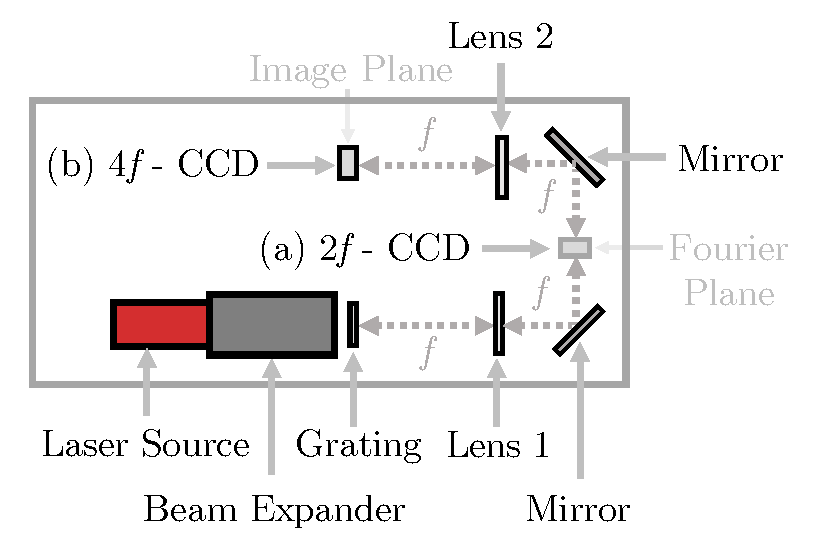
\includegraphics[width=6.5cm]{method/fig1-1}
\caption[]{A plan view schematic of the experimental set-up used to collect data. $f$ is the focal length distances of the lenses. Each component was attached to an optical breadboard. (a) Represents the main $2f$ optical system used where the majority of data was collected. (b) Represents the 'standard' $4f$ optical system.}
\label{m-fig1}
\end{center}
\end{figure}

A coherent laser source of wavelength $\sim635$ nm was used as our source of radiation. A $\times10$ beam expander was placed directly after this to allow the beam width to be adjusted during experimentation, this was done so that the majority of the light would strike the area of the diffraction grating.

To place the lenses at the correct distances their focal lengths had to be measured. This was done by placing each lens at the beam expander, a screen was then moved closer and further away from the source until the brightest and sharpest spot could be observed. At that distance was thus the focal length, measured with a metre ruler we found that for both lens 1 and 2, their focal lengths were $48\pm1$ cm.

Due to the constraint with the size of the breadboard, mirrors were used to reflect the light so that the set-up would take up less space. Two were positioned so that light could be reflected into a CCD camera, and ensuring that the focal length distances were preserved.

This camera was moved at various stages of experimentation, from being in the Fourier plane at a distance of $2f$ to $4f$ when we wanted observations made in the Image plane.

Our CCD was controlled using the manufacturer's software, images were saved and then later analysed using modules compiled in Python and in MATLAB. The outputs contained an intensity map of a grayscale version of the image, and intensity profiles of the $x$ and $y$ directions of the intensity map.  

The grayscale images were obtained by converting each pixel from sRGB into a singular value defined by the CIE 1931 Linear Luminance,
\begin{equation}
Y_{\text{linear}}=0.2126R+0.7152G+0.0722B,
\end{equation}

where $R,G,B$ are the respective \textit{red}, \textit{green}, and \textit{blue} values of a pixel \cite{rgbtogray}. This equations limits the range of the value that a pixel could hold, from 0 to 255. Where 0 is equations to being completely dark to 255 which means that the maximum amount of light can be achieved.

The intensity profiles were created by averaging the rows or columns within the images that contained the greatest amount of pixels with values of 255. When averaged together a standard deviation could be found and then subsequently a $\chi^2$ value could be calculated when a theoretical model was compared to the intensity graphs.

Throughout our research we varied the gratings that were used, the diffraction gratings were placed within a holder just after the beam expander and the pattern that they created was observed at different distances. 

Adjustments had to be made to the set-up so that the pattern observed was as clear as possible. A recurring problem was the over-saturation of the features in the diffraction pattern. This was corrected by using a neutral density filter, adjusting the exposure time and the gain of the CCD within the software.

To measure small scale distances of features on the diffraction grating, a travelling microscope with a Vernier scale was used.

\vspace{-3ex}
\section{Results}
\vspace{-2ex}
Figure \ref{horizontal_profiles} show multiple plots of the horizontal intensity graph in the Fourier plane against the distance along the $x$ direction for different diffraction patterns.
\begin{figure}[!h]
\begin{center}
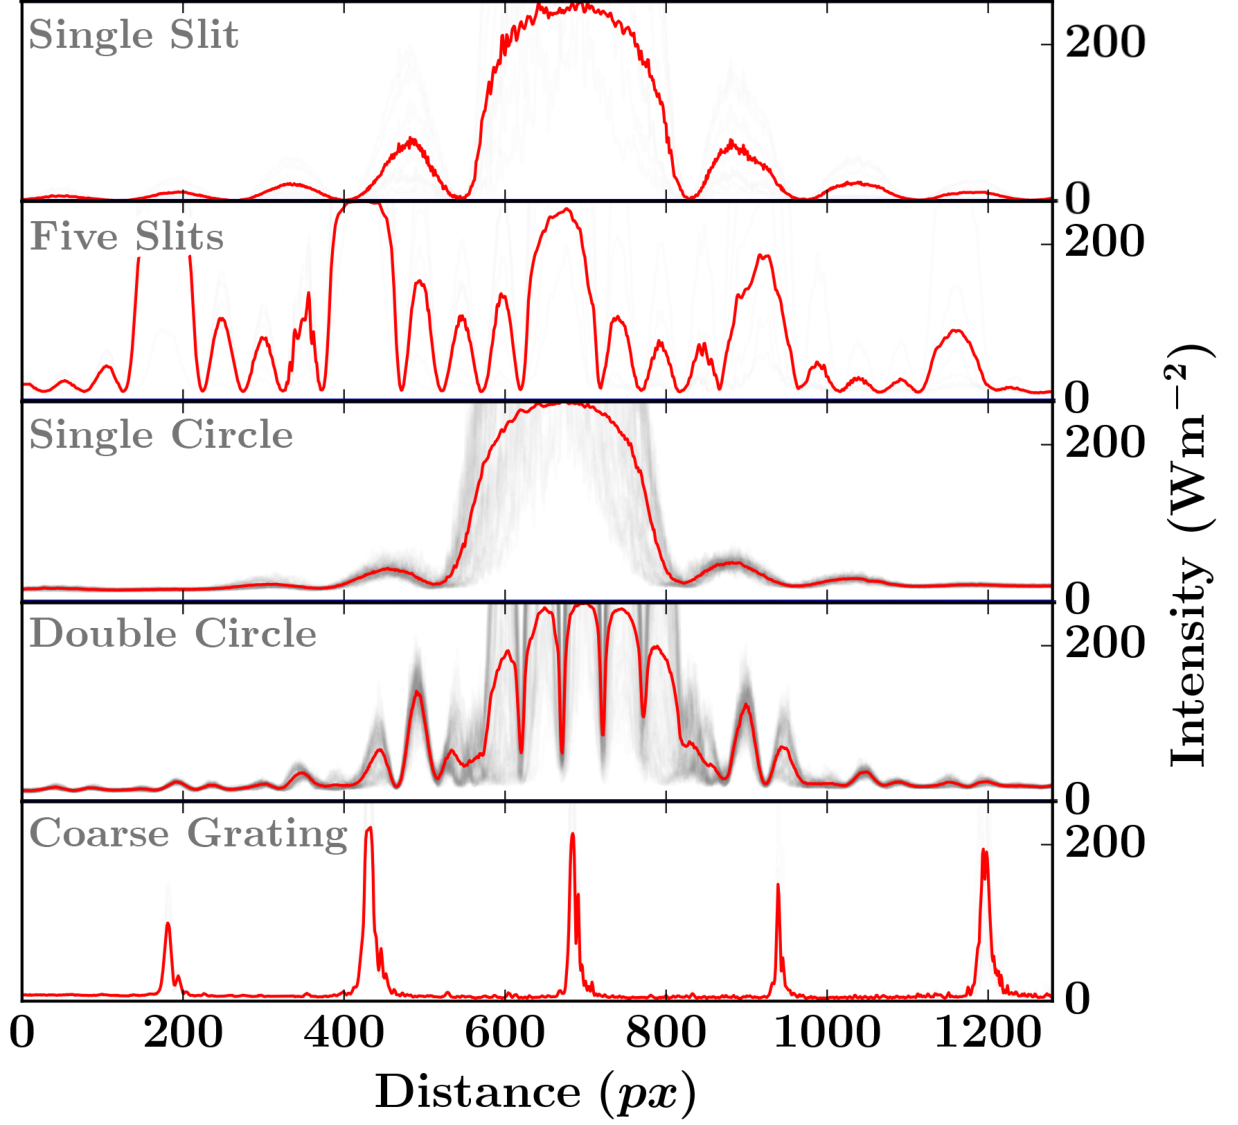
\includegraphics[width=7cm]{results/horizontal_intensity_profiles}
\caption[]{The horizontal intensity profiles of diffraction patterns within the Fourier plane created with different diffraction gratings. The grey shadow behind the main diagrams are the graphs that were average to create the profile that is shown. The intensity ranges from 0 to 256.}
\label{horizontal_profiles}
\end{center}
\end{figure}

\begin{figure}[!h]
\begin{center}
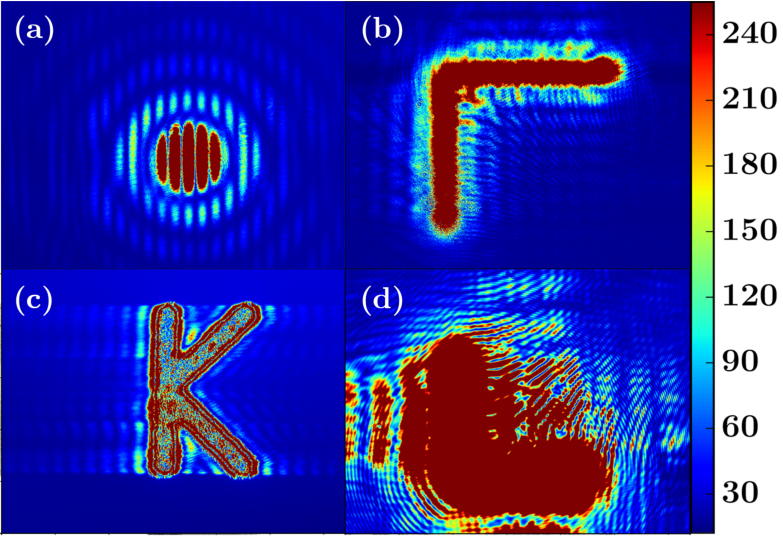
\includegraphics[width=9cm]{results/collage}
\caption[]{Intensity maps of four different diffraction patterns taken from different planes: (a) double circle grating in Fourier plane, (b) L grating in image plane, (c) K grating in image plane which has been low-passed filtered, (d) L grating in '$3f$' plane.}
\end{center}
\end{figure}

More results

\begin{figure}[!h]
\begin{center}
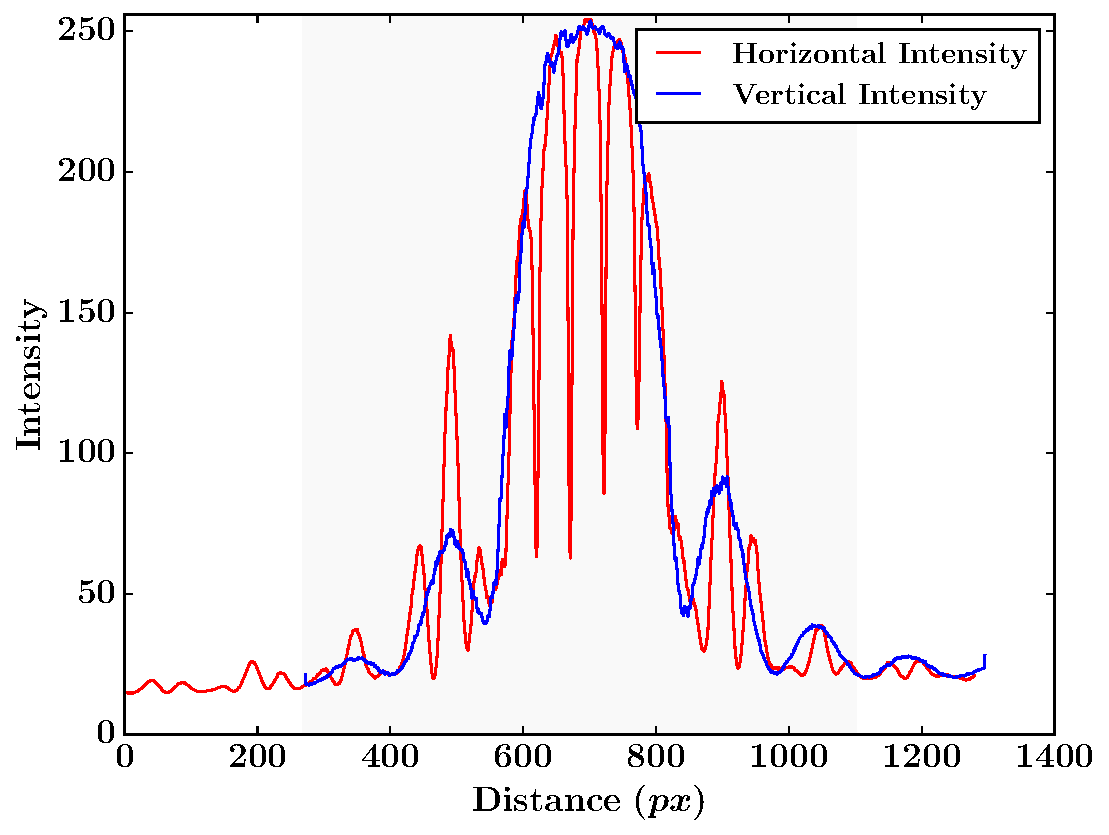
\includegraphics[width=9cm]{results/double_circle_intensity_overlapped}
\caption[]{Overlapped intensity profiles of the $x$ and $y$ direction for the double circular aperture. This highlights the envelope nature of the intensities?}
\end{center}
\end{figure}

\begin{table}[h!]
\centering
\begin{tabular}{c@{\hskip 20pt}c@{\hskip 20pt}c@{\hskip 20pt}c} 
 \hline
 \textbf{Grating} & $\boldsymbol{\chi^2}$ \\ [0.5ex] 
 Single Slit &$36.8$ \\ 
 Five Slits & $-$ \\
 Double Circle & $-$ \\
 \hline
\end{tabular}
\caption{A theoretical model was applied to the single slit, five slits, and double circle diffraction gratings. Only the single slit provided a fit that would allow us to calculate a $\chi^2$ value.}
\end{table}

\begin{table}[h!]
\centering
\begin{tabular}{c@{\hskip 15pt}c@{\hskip 15pt}c@{\hskip 10pt}c} 
 \hline
 \textbf{Grating} & \textbf{Real Space [mm]} & \textbf{Fourier Space [mm]} \\ [0.5ex] 
 $1$ &$0.20\pm0.01$ & $0.11\pm0.03$ \\ 
 $2$ & $0.12\pm0.01$ & $0.11\pm0.01$ \\
 $3$ & $0.08\pm0.01$ & $0.05\pm0.01$ \\
 \hline
\end{tabular}
\caption{For each coarse diffraction grating, the diffraction grating slit width is shown as measured in real space, and as calculated in Fourier space.}
\end{table}

\vspace{-3ex}
\section{Discussion}
\vspace{-2ex}
From our results we see that 

\Blindtext

\vspace{-5ex}
\section{Conclusions}
\vspace{-2ex}

Conclusion

\blindtext

\begin{thebibliography}{5}
\bibitem{mathmethods}
	K. F. Riley, M. P. Hobson, and S. J. Bence.
	\textit{Mathematical Methods for Physics and Engineering}.
	Cambridge University Press, Cambridge, UK, 2010.
	
\bibitem{of2f}
	C. S. Adams and I. G. Hughes.
	\textit{Optics f2f, from Fourier to Fresnel}.
	Clarendon Press, Oxford, UK, 2017.

\bibitem{elecdiffraction}
	K. W. Andrews, D. J. Dyson, and S. R. Keown.
	\textit{Interpretation of Electron Diffraction Patterns}.
	Hilger \& Watts Ltd, London, UK, 1967.
	
\bibitem{xraypharma}
	J. P. Smit, R. B. McClurg.	
	\textit{X-ray Powder Diffraction Pattern Indexing for Pharmaceutical Applications}.
	Pharmaceutical Technology, January 2013, Vol. 37, No. 1.
	
\bibitem{singleslit}
	A. R. Lang, et al.
	\textit{Single-slit diffraction patterns of sub-nanometre-wavelength synchrotron radiation}.
	Journal of Physics D: Applied Physics, 1987, Vol. 20, No. 4, pp. 541-544.
	
\bibitem{xrayphase}
	S. C. Mayo, et al.
	\textit{X-ray phase-contrast microscopy and microtomography}.
	Optical Express, 2003, Vol. 11, No. 19, pp. 2289-2302.
	
\bibitem{rgbtogray}
	M. Stokes, et al.
	\textit{A Standard Default Color Space for the Internet}.
	November 1996, available at: https://www.w3.org/Graphics/Color/sRGB, accessed: 11th February 2017. 

\bibitem{youngandfreedman} 
	Hugh D. Young and Roger A. Freedman.
	\textit{University Physics with Modern Physics, 13th Edition}. 
	Pearson Education Limited, Essex, UK, 2015.
	
\bibitem{hughesandhayes} 
	I. G. Hughes and T. P. A. Hase.
	\textit{Measurements and their Uncertainties}. 
	Oxford University Press, Oxford, UK, 2010.
	
\end{thebibliography}
\clearpage

\vfill
\twocolumngrid
\vspace{-3ex}
\section*{Appendix}
\vspace{-2ex}

Appendix


\clearpage
\end{document}